% ! TeX root = ../../master-thesis.tex

\section{Finite Stream Extension}
\label{section:implementation:finite-stream-extension}

Another extension implemented for the Sodium library is the
\texttt{FiniteStreamExten\-sion}, which defines a new type of reactive variable
derived from \texttt{Stream}s, namely the \texttt{Finite\-Stream} type, as
illustrated in Figure \ref{figure:finite-stream-extension-class-diagram}.

\begin{figure}[!ht]
  \centering
  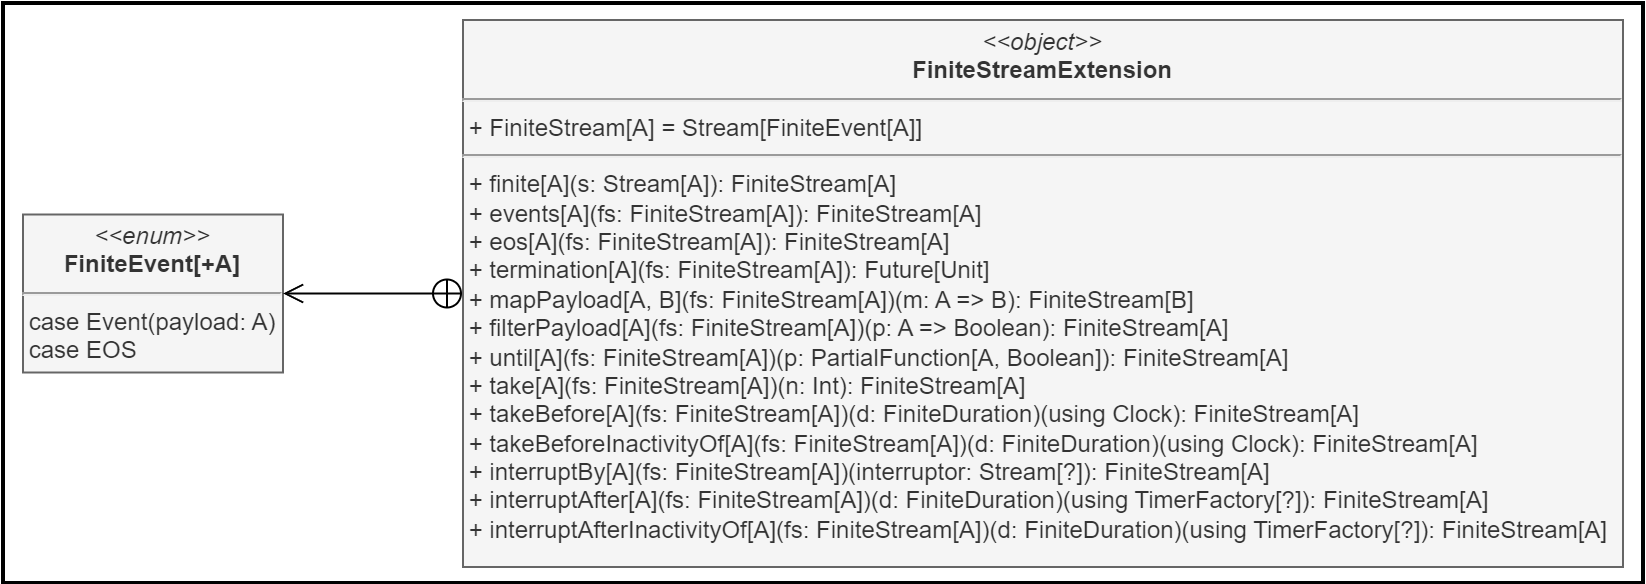
\includegraphics[width=1\textwidth]{resources/figures/finite-stream-extension-class-diagram.png}
  \caption{
    A UML class diagram of the \texttt{FiniteStream} extension
    and its operators.
  }
  \label{figure:finite-stream-extension-class-diagram}
\end{figure}

In Sodium, \texttt{Stream}s may fire new events indefinitely, making them
suitable for modelling any type of producer. However, in their generality,
\texttt{Stream}s do not capture directly the fact that some producers only emit
a finite amount of events. For this purpose, \texttt{FiniteStream}s have been
designed to fire a finite amount of events before notifying all the dependents
of their termination.

Since extending \texttt{Stream}s is not allowed in Sodium,
\texttt{FiniteStream}s have been implemented as \texttt{Stream}s of
\texttt{FiniteEvent}s, which can either be \texttt{Event}s, wrapping a payload,
or an \texttt{EOS (End Of Stream)}, marking the termination of the stream. This
implementation allows leveraging the \texttt{Stream} operators also for
\texttt{FiniteStream}s, however, it does not restrict producers from emitting
additional events after the first \texttt{EOS}. To solve this problem, every
event following the first \texttt{EOS} is automatically discarded.

The \texttt{FiniteStreamExtension} provides a set of operators for creating
\texttt{Finite\-Stream}s, implemented in the form of Scala's extension methods,
similarly to the \texttt{StreamExten\-sion}. For better compositionality, these
operators have been designed to transform \texttt{FiniteStream}s into other
\texttt{FiniteStream}s. In fact, if the operators were transformations from
\texttt{Stream}s to \texttt{FiniteStream}s, they would wrap the firings of an
input \texttt{Stream} inside the \texttt{FiniteEvent}s of an output
\texttt{FiniteStream}. However, they could also be applied to
\texttt{FiniteStream}s, wrapping the \texttt{Finite\-Event}s of an input
\texttt{FiniteStream} inside the \texttt{FiniteEvent}s of an output
\texttt{Finite\-Stream}. As a consequence, any combination of operators would
create a \texttt{Stream} of nested \texttt{FiniteEvent}s, requiring recursive
unnesting to access the actual payload of the events. For this reason, the only
operator converting \texttt{Stream}s into \texttt{FiniteStream}s is the entry
point of the extension, namely the \texttt{finite} operator, which simply wraps
any event of an input \texttt{Stream} inside an \texttt{Event} of an output
\texttt{FiniteStream}.

The sole purpose of \texttt{finite} is to enable the application of the other
operators of the extension, namely:
\begin{itemize}
  \item \texttt{until}: when applied to an input \texttt{FiniteStream} $s$,
        return an output \texttt{Finite\-Stream} $s'$, obtained by halting $s$
        at the first event whose payload satisfies a given \texttt{predicate}.
  \item \texttt{take}: when applied to an input \texttt{FiniteStream} $s$,
        return an output \texttt{Finite\-Stream} $s'$, obtained by halting $s$
        after a given number of events.
  \item \texttt{interruptBy}: when applied to an input \texttt{FiniteStream}
        $s$, return an output \texttt{FiniteStream} $s'$, obtained by halting
        $s$ at the first event of a given \texttt{interruptor} stream.
  \item \texttt{takeBefore}: when applied to an input \texttt{FiniteStream}
        $s$, return an output \texttt{FiniteStream} $s'$, obtained by halting
        $s$ at the first event fired after a given \texttt{duration} has
        elapsed since the creation of $s'$.
  \item \texttt{interruptAfter}: when applied to an input \texttt{FiniteStream}
        $s$, return an output \texttt{FiniteStream} $s'$, obtained by halting
        $s$ after a given \texttt{duration} has elapsed since the creation of
        $s'$. The operator relies on a \texttt{Timer} to generate a
        notification after a set amount of time.
  \item \texttt{takeBeforeInactivityOf}: when applied to an input
        \texttt{FiniteStream} $s$, return an output \texttt{FiniteStream} $s'$,
        obtained by halting $s$ at the first event fired after a given
        \texttt{duration} has elapsed since its latest event.
  \item \texttt{interruptAfterInactivityOf}: when applied to an input
        \texttt{FiniteStream} $s$, return an output \texttt{FiniteStream} $s'$,
        obtained by halting $s$ after a given \texttt{duration} has elapsed
        since its latest event. The operator relies on a \texttt{Timer},
        similarly to \texttt{interruptAfter}.
\end{itemize}

An example of application of the \texttt{FiniteStreamExtension} is the
implementation of several \texttt{HaltPolicy}s for simulations, including
\texttt{haltAfterDurationOf} and \texttt{haltAfterInactivityOf} for concurrent
simulations.
